% NEWLY INSERTED SECTION: DSL Overview, CLI, Frontend, API, and Technical Implementation
\refstepcounter{chapter}
\chapter*{Implementation}
\phantomsection
\addcontentsline{toc}{chapter}{Implementation}
\label{ch:incidentflow_architecture}

This chapter details the design, structure, and implementation of IncidentFlow, describing how the CLI, frontend, and HTTP API work together to enable automated incident response documentation.

The IncidentFlow ecosystem is built upon a modular architecture, separating the core language compilation from the user-facing interfaces. At the parser level, ANTLR leverages the \texttt{IncidentFlow.g4} grammar definition to translate the source text into a deeply nested Parse Tree. The sequence of language tokens navigates through the lexer to extract fundamental constructs representing triggers and phases. 

The compiler traverses this tree, checking block topologies and identifying invalid state jumps (e.g., verifying that \texttt{GOTO} expressions route securely to instanced blocks). During compilation, the engine tracks concurrent definitions encapsulated in \texttt{PARALLEL} directives, mapping them coherently to report structures rather than raw serialized logging commands. Wait behaviors map cleanly into distinct timeline expectations inside the final Markdown string. The report generation logic fundamentally hinges on a template translation pattern parsing the semantic tree sequentially, generating Markdown header blocks, and rendering an accumulative trail of \texttt{SEVERITY} adjustments.

\subsection{Command-Line Interface (CLI)}
\label{subsec:impl_cli}

The \texttt{iflow} command serves as the primary entry point for interacting with the compiler toolkit. To deploy the toolchain, users can execute the provided \texttt{install.sh} script from the project root, which globally registers the wrapper within the local binary paths. Alternatively, it can be executed natively from the source directory via \texttt{./iflow <command>}.

Once established, the CLI exposes a diverse suite of workflows tailored to validation, active processing, and interactive generation. 

At the foundational validation level, the \texttt{check} command evaluates a provided playbook for both syntax compliance against the ANTLR grammar and deeper semantic consistency. For example, executing:
\begin{lstlisting}[language=bash]
$ iflow check playbooks/sample.iflow
  -> Checking playbooks/sample.iflow ...
  O: No errors found.
\end{lstlisting}
guarantees that the underlying state machine is well-formed. Crucially, the semantic checks verify constraints such as ensuring all \texttt{GOTO} execution jumps reference strictly existing and valid phases. When clean, the process exits with code 0; otherwise, it predictably terminates with codes 2 or 3 depending on whether it failed syntactically or semantically.

Once a playbook is verified, the \texttt{report} command orchestrates the compilation pipeline, translating the technical response script into a structured Markdown document. This generated report encompasses configuration schemas, phase-by-phase action breakdowns, explicit logging entries, and an accumulative severity evolution trail. By default, running a report prints the Markdown payload directly to the standard output:
\begin{lstlisting}[language=bash]
$ iflow report playbooks/phishing.iflow
  # Incident Report
  ## Phishing Details...
\end{lstlisting}
Redirecting this output to an artifact file is natively supported via the \texttt{-o} flag (e.g., \texttt{iflow report playbooks/phishing.iflow -o out.md}).

To accelerate incident response workflows during high-pressure scenarios, the CLI provides an advanced interactive \texttt{wizard} command. Rather than demanding engineers to write raw DSL code from scratch, starting an interactive session sequentially queries the analyst regarding incident symptoms and evidence. The engine prompts for specific MITRE ATT\&CK classifications, currently encompassing T1566 (Phishing), T1059.001 (PowerShell Execution), and T1055 (Process Injection).

\begin{lstlisting}[language=bash]
$ iflow wizard

  Select the attack technique:
    1) T1566     - Phishing
    2) T1059.001 - PowerShell Execution
    3) T1055     - Process Injection
  > 1

  Output base name: > phishing_incident

  What severity level triggered this alert?
    1) LOW  2) MEDIUM  3) HIGH  4) CRITICAL
  > 3
\end{lstlisting}
By feeding numerical prompts back into the console, the wizard transpiles those decisions directly into dual artifacts: a pristine \texttt{.iflow} playbook script and a compiled Markdown report.

Beyond standalone task execution, the CLI embeds diagnostic and integration features. Developers can invoke the \texttt{tree} command to visually spawn a GUI representing the topological parse tree. This greatly aids grammar diagnostics when extending the incident language:
\begin{lstlisting}[language=bash]
$ iflow tree playbooks/sample.iflow
  -> Launching AST visualizer...
\end{lstlisting}

For API-first ecosystems, the \texttt{serve} command dynamically spawns the HTTP API discussed subsequently. This background service abstracts the CLI layer entirely:
\begin{lstlisting}[language=bash]
$ iflow serve -p 8080 -d playbooks/
  -> Starting HTTP API on port 8080...
  -> Watching directory: playbooks/
\end{lstlisting}
This backend accepts target port (\texttt{-p}) and active playbook directory (\texttt{-d}) arguments, providing a foundational bridge for the React and Vite frontend.
\subsection{HTTP API Backend}
\label{subsec:impl_api}

To facilitate interactions from the frontend and external tools, the IncidentFlow compiler operates as a dynamic background service via the \texttt{iflow serve} command. It exposes a lightweight JSON REST API routing compilation tasks without the overhead of the CLI environment.

Crucial endpoints include:
\begin{itemize}
    \item \texttt{POST /api/compile}: Accepts arbitrary \texttt{.iflow} strings, funneling them through the parser and returning \texttt{\{ "valid": true \}} on success, or structured error arrays on internal failure.
    \item \texttt{POST /api/report}: Runs the validations and appends a \texttt{report} JSON key encapsulating the final formatted Markdown string.
    \item \texttt{GET /api/playbooks}: Discovers all pre-existing \texttt{.iflow} files allocated in the server's working directory, enabling templates to be queried algorithmically.
\end{itemize}

A valid code compilation guarantees an HTTP 200 OK. For example, verifying a valid syntax snippet returns a successful boolean mapping:
\begin{lstlisting}[language=java]
// POST /api/compile Request
{
  "code": "PLAYBOOK \"Demo\" \n TRIGGER \"Alert\" \n PHASE Initial {}"
}

// Response (200 OK)
{
  "valid": true,
  "errors": []
}
\end{lstlisting}

Conversely, malformed source texts yield an HTTP 422 Unprocessable Entity combined with explicit parser notifications detailing the broken token and its precise line or character location:
\begin{lstlisting}[language=java]
// Response (422 Unprocessable Entity)
{
  "valid": false,
  "errors": [
    "line 3:0 mismatched input 'PHASE' expecting 'TRIGGER'"
  ]
}
\end{lstlisting}

To bridge natively with the visual web interface, CORS (Cross-Origin Resource Sharing) support is compiled directly into the API runtime, enabling decoupled frontend environments to execute HTTP calls directly from the user's browser securely.

\subsection{Frontend Architecture and UI}
\label{subsec:impl_frontend}

The IncidentFlow frontend is built using React and Vite. It serves as a visual client that communicates with the HTTP API for code compilation and validation, eliminating the need to install the CLI locally. 

The application layout centers around a text editor for the DSL alongside a real-time Markdown preview window (see Figure~\ref{fig:ui_main}). 

\begin{figure}[htbp]
    \centering
    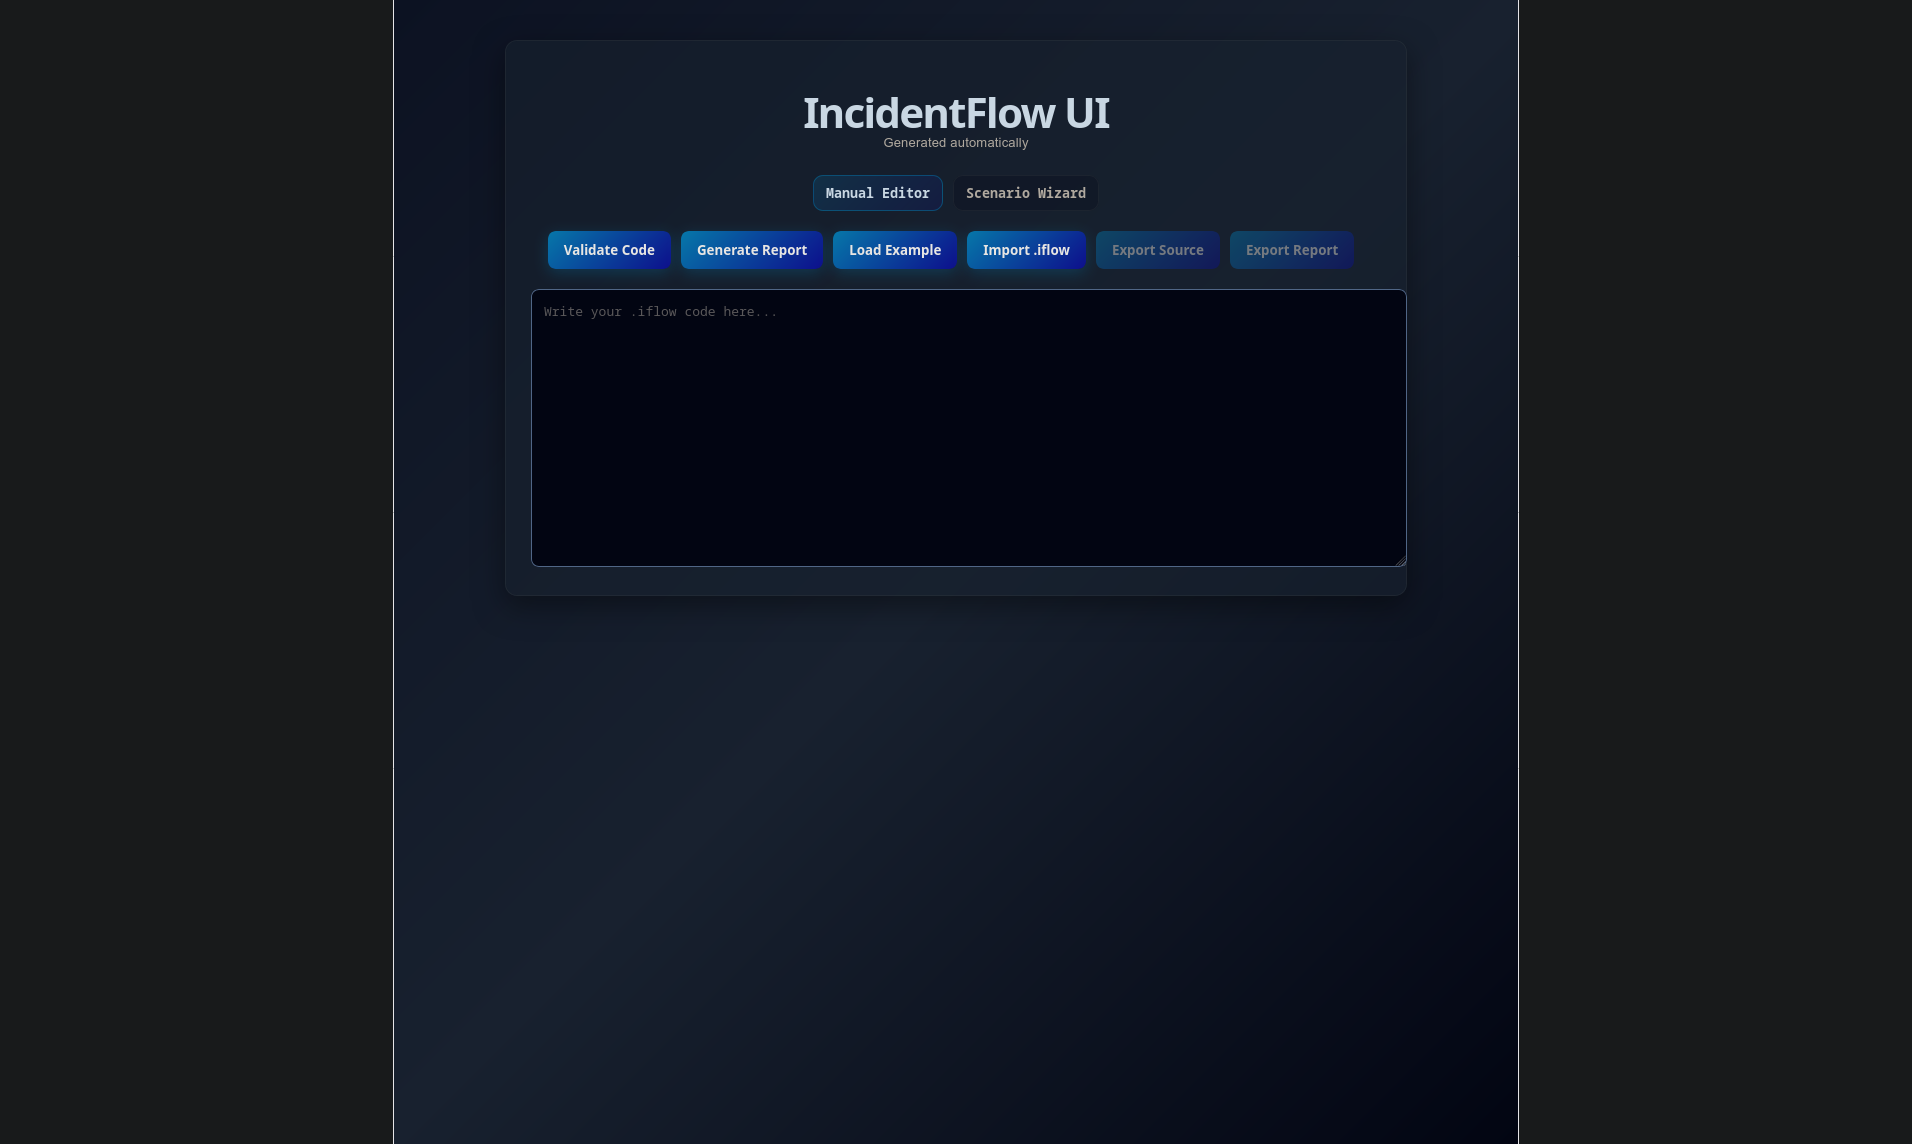
\includegraphics[width=0.8\textwidth]{images/main_page.png}
    \caption{The main editor interface of the IncidentFlow UI.}
    \label{fig:ui_main}
\end{figure}

The application state is managed using standard React hooks. When users type in the Manual Editor, the input is stored in a component state. To avoid overloading the backend with validation requests on every keystroke, a debouncing effect delays the API call until the user pauses typing. The frontend sends the content to the \texttt{/api/compile} endpoint and updates the UI based on the response.

Error processing is handled dynamically. When the API returns an HTTP 422 status code, the frontend extracts the error array and renders it below the editor. This translates terminal-based tracebacks into immediate visual feedback:
\begin{lstlisting}[language=HTML]
<div className="error-banner">
  Syntax Error at Line 12: Unexpected token 'GOTO'
</div>
\end{lstlisting}

In addition to manual authoring, the frontend implements a visual form to guide users through report generation called the "Scenario Wizard" (illustrated in Figure~\ref{fig:ui_wizard}). 

\begin{figure}[htbp]
    \centering
    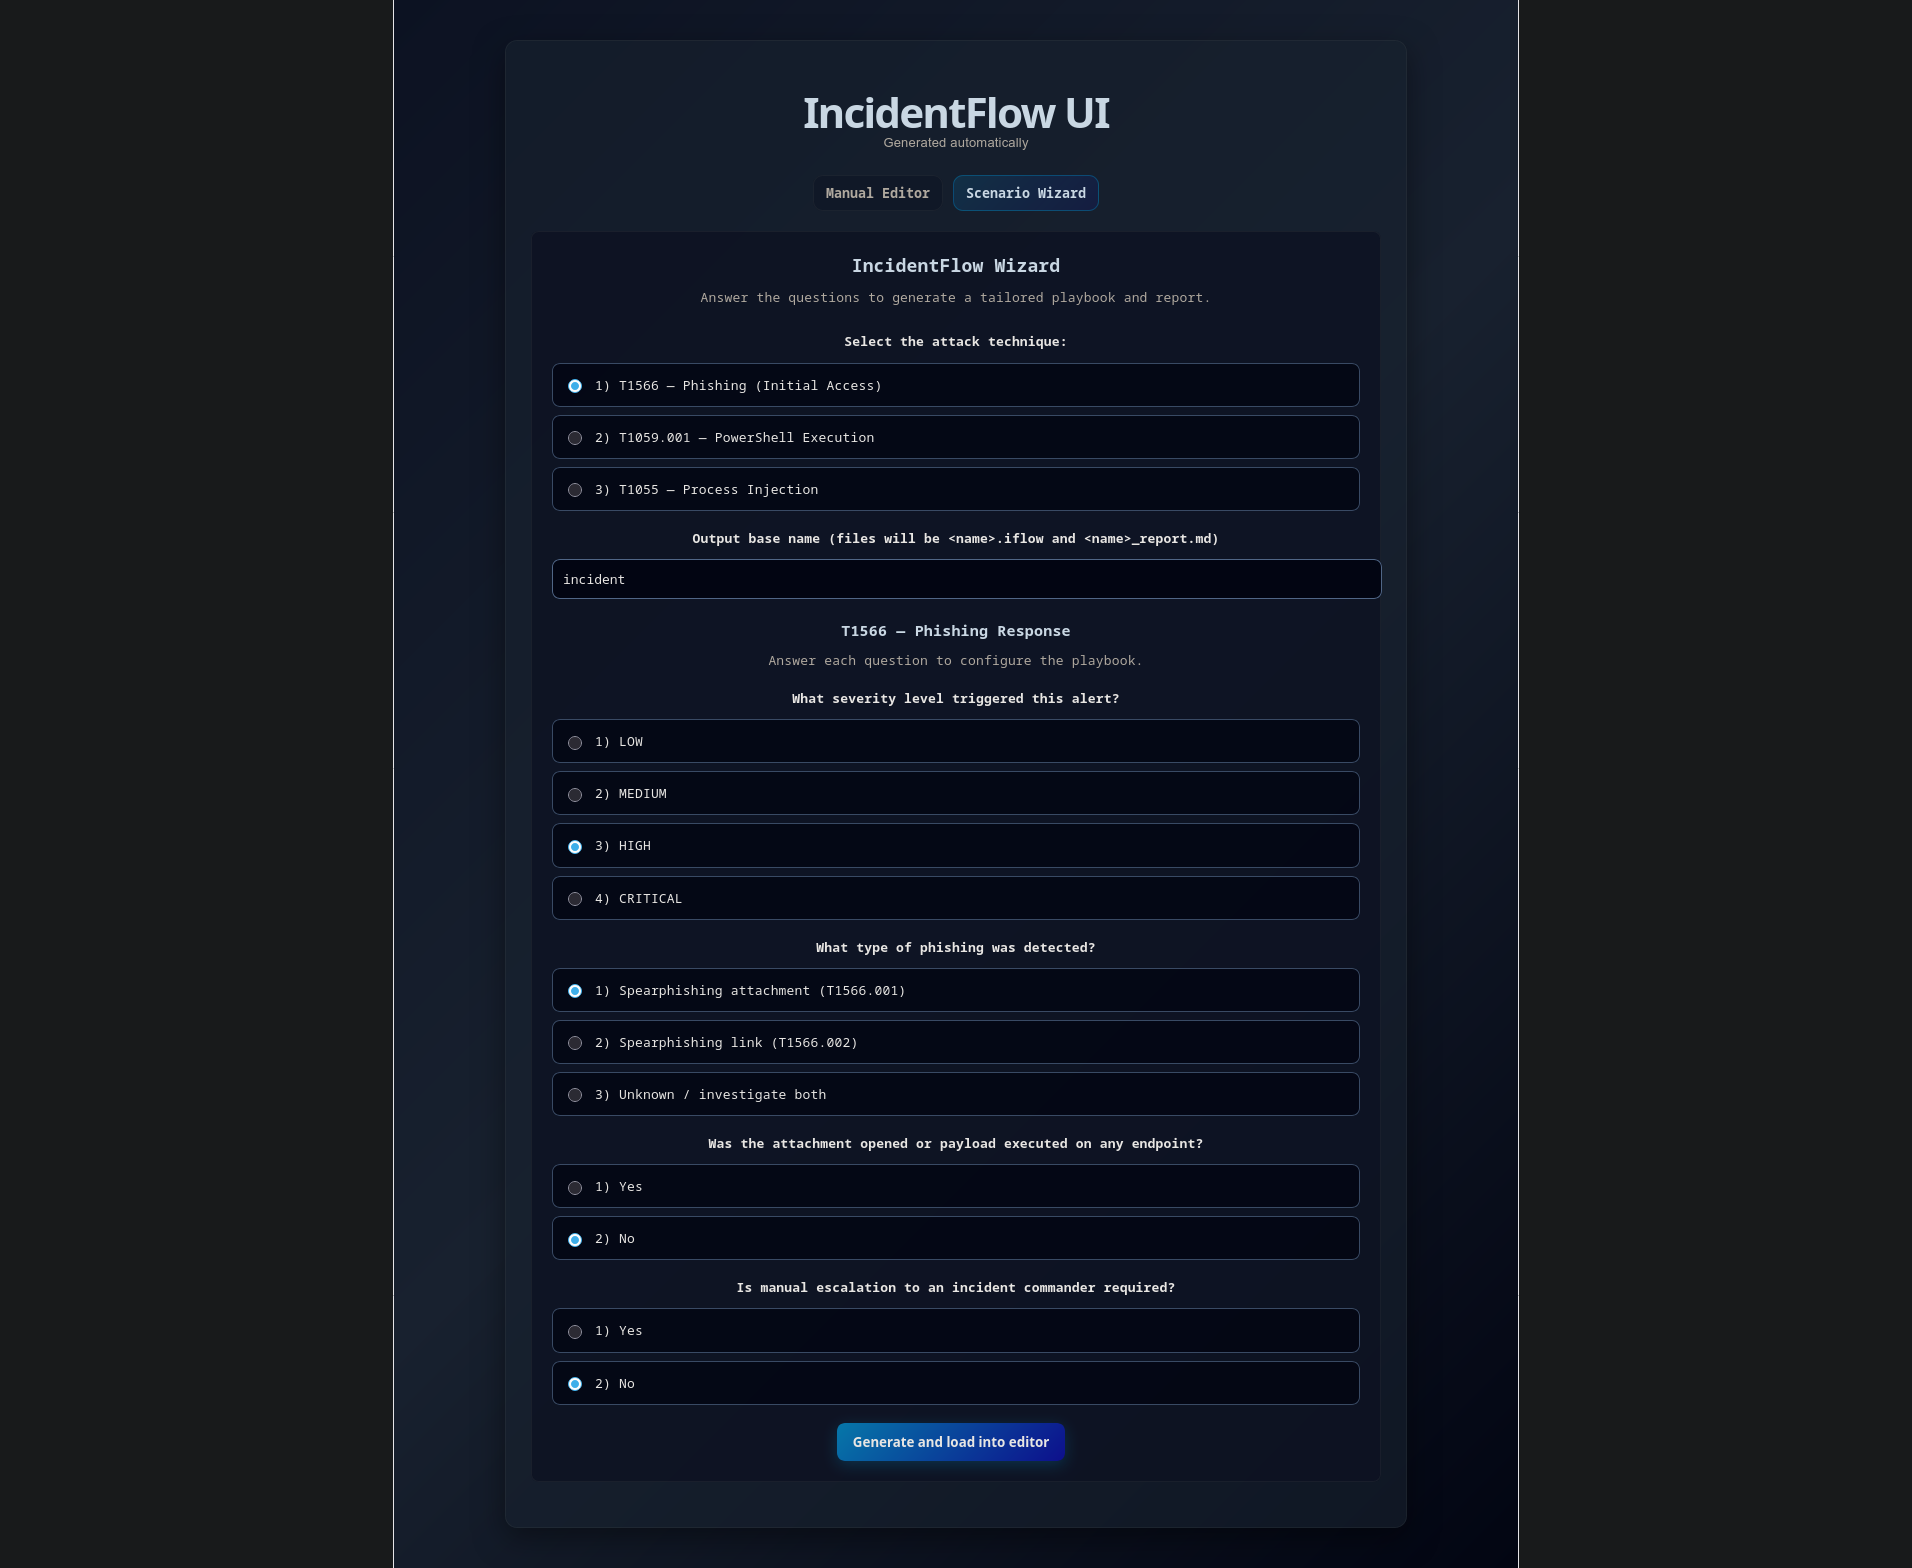
\includegraphics[width=0.8\textwidth]{images/scenario_wizard.png}
    \caption{The interactive Scenario Wizard.}
    \label{fig:ui_wizard}
\end{figure}

This wizard replicates the interactive command-line prompts by iterating through a series of predefined questions regarding the incident, such as MITRE ATT\&CK classifications and threat severity. The collected answers are then formatted into valid DSL code and sent directly to the compiler.

For users who prefer modifying existing playbooks, the interface includes a template loader. This feature queries the \texttt{/api/playbooks} REST endpoint and presents available scripts in a dropdown menu (shown in Figure~\ref{fig:ui_example}).

\begin{figure}[htbp]
    \centering
    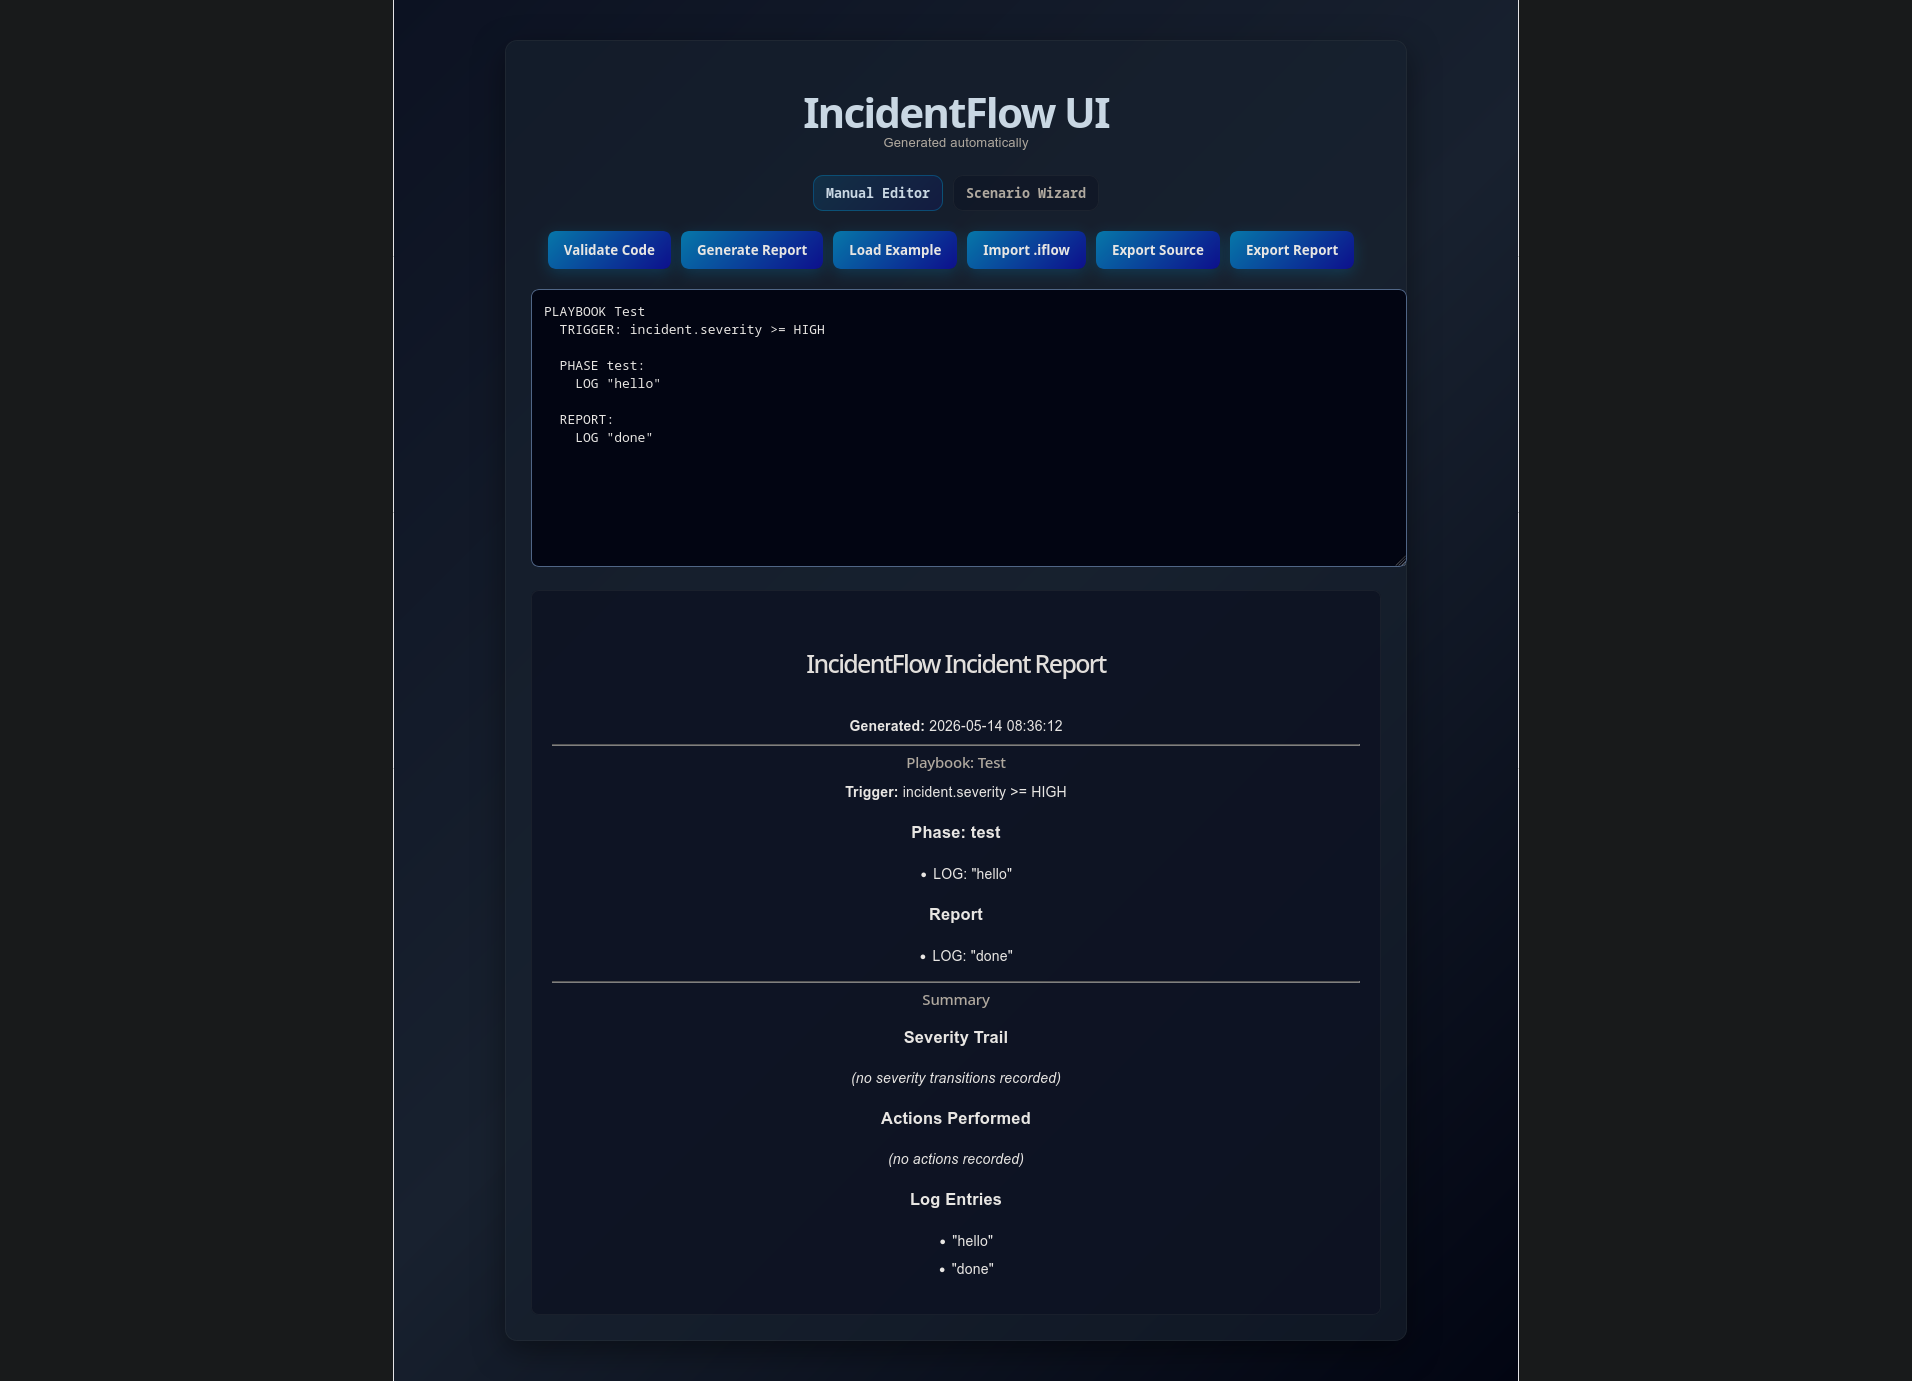
\includegraphics[width=0.8\textwidth]{images/generate_report_using_example.png}
    \caption{Loading and browsing playbook examples.}
    \label{fig:ui_example}
\end{figure}

Selecting an example overwrites the editor's current state with the loaded string, triggering an automatic re-compilation.

Finally, when the DSL code is valid, the frontend requests the final report representation via the \texttt{/api/report} endpoint. The JSON response contains a rendered Markdown string. The frontend passes this string to a React Markdown parser, producing a styled HTML document that the user can immediately export or copy (Figure~\ref{fig:ui_report_gen}).

\begin{figure}[htbp]
    \centering
    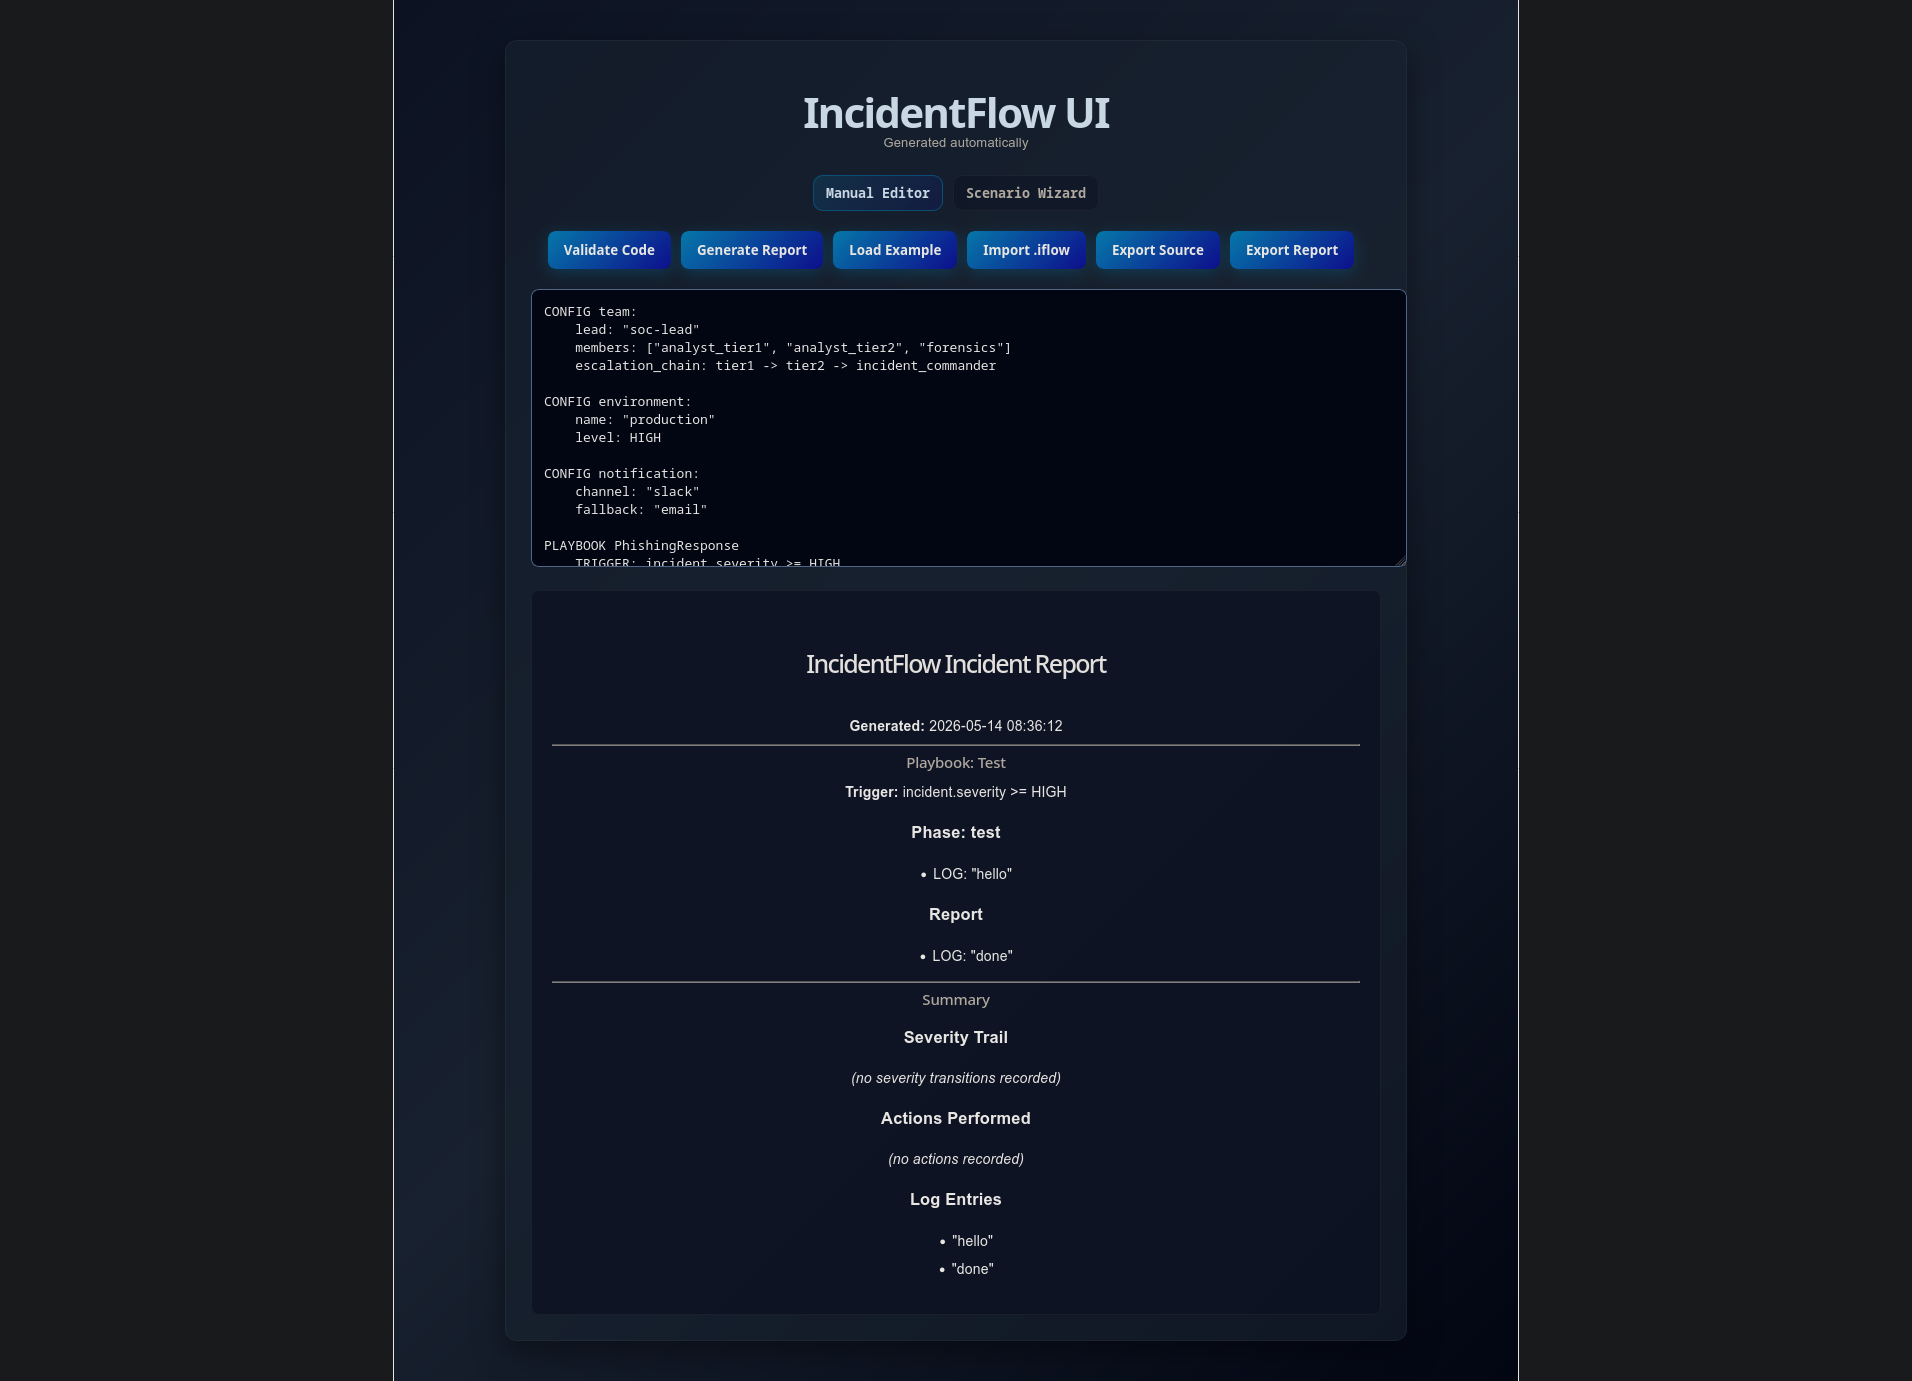
\includegraphics[width=0.8\textwidth]{images/generated_report_using_wizard.png}
    \caption{The resultant incident report rendered visually next to the editor.}
    \label{fig:ui_report_gen}
\end{figure}
